\documentclass{article}
\usepackage{graphicx}
\usepackage{hyperref}
\usepackage{booktabs}
\usepackage{multirow}
\usepackage{siunitx}
\usepackage[letterpaper,margin=0.75in]{geometry}
\usepackage[font=small,skip=-1pt]{caption}
\usepackage{amssymb}
\usepackage{amsmath}

%%%%%%%%%%%%%%%%%%%%%%%%%%%%%%%%%%%%%%%%%%%%%%%%%%%%%%%%%%%%%
%  This is a special package and its settings for displaying computer code in a LaTeX file
%
\usepackage{listings}
\usepackage{float}
\lstset{ %
language=R,
basicstyle=\footnotesize,
numbers=left,
numberstyle=\footnotesize,
stepnumber=1,
numbersep=5pt,
showspaces=false,
showstringspaces=false,
showtabs=false,
frame=single,
tabsize=2,
captionpos=b,
breaklines=true,
breakatwhitespace=false,
escapeinside={\%*}{*)}
}

%%%%%%%%%%%%%%%%%%%%%%%%%%%%%%%%%%%%%%%%%%%%%%%%%%%%%%%%%%%%%%
\title{{\sffamily Finite Difference Derivatives} \\ 
{\sc CLA 365 technical report }}

\author{Charles Zhang \and Emil Bao Le \and Henry Bell \and Zuofu Huang}
\date{\today}

\begin{document}
\maketitle

\begin{abstract} 

\noindent In this report, we present R code that implement methods for approximating the derivatives of continuous functions. We implement function D using the forward difference method. Based on function D, we update our Newton's method so that the derivative is computed within Newton's method instead of inputted. We then discuss the drawbacks of the forward-difference method and produce a comparison between forward-difference, backwards difference and three-point centered-difference method.

\end{abstract}
\section*{Introduction}

The derivative is widely used in exploring the global and local behavior of functions. We implement finite difference methods to numerically find derivatives in R. We also investigate $\delta$ values that minimize errors and perform cross-method comparisons among forward difference, backward difference and three-point centered difference methods.

\section{Derivative Function}
\subsection{Overview}

Our derivative function is based on the method of finite differences.
The method of finite differences builds on the concept that the slope is $\frac{\Delta y}{\Delta x}$. Assuming $f$ is continuous, $\frac{\Delta y}{\Delta x}$ can be approximated by $\frac{f(x_ + \delta) - f(x)}{\delta}$ where $\delta \in \mathbb{R}$. The accuracy of our approximation of the slope (denoted $f^{\prime}$) improves as $\delta \rightarrow 0$. This is only one of three finite difference methods, the others will be discussed later in the paper. This one is called the forward method. \\

\begin{equation}
f^{\prime}(x)=\lim \limits_{\delta\rightarrow0}\frac{f(x-\delta)-f(x)}{\delta}
\end{equation}

\subsection{Implementation}

\begin{lstlisting}
D <- function(f, delta=.001) {
  result <- function(x) (f(x+delta)-f(x))/delta
  return(result)
}
\end{lstlisting}
\noindent
\subsection{Testing}
We tested our derivative on a function whose derivative is known: $f(x) = x \cdot e^{-x^2}$. Figure 1 plots the original function $f(x)$.Figure 2 plots the function's derivative computed with function D.

\begin{figure}[H]
   \begin{minipage}{0.48\textwidth}
     \centering
     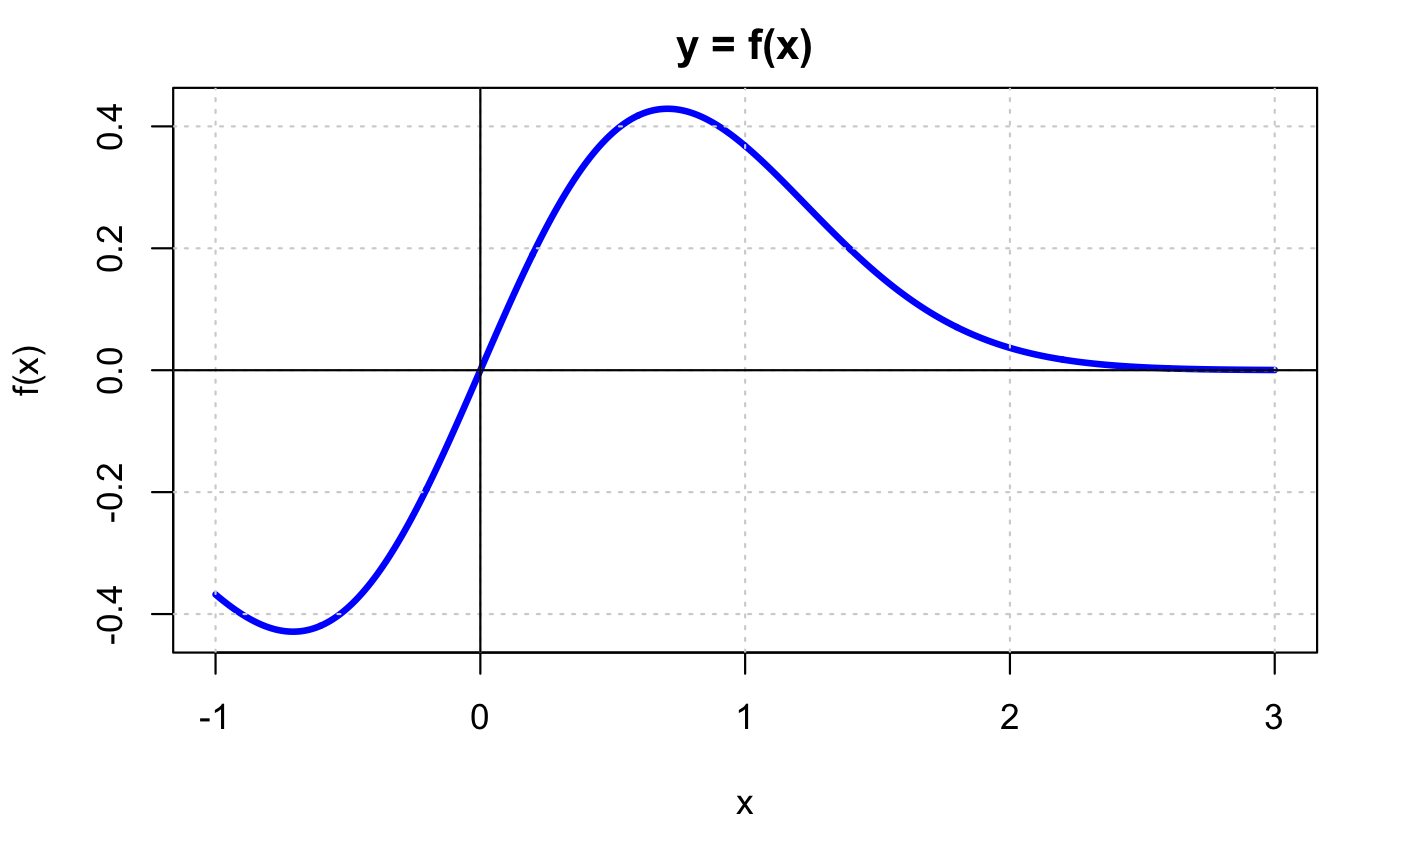
\includegraphics[width=.99\linewidth]{dx.png}
     \caption{$f(x) = xe^{-x^2}$}\label{Fig:Data1}
   \end{minipage}\hfill
   \begin{minipage}{0.48\textwidth}
     \centering
     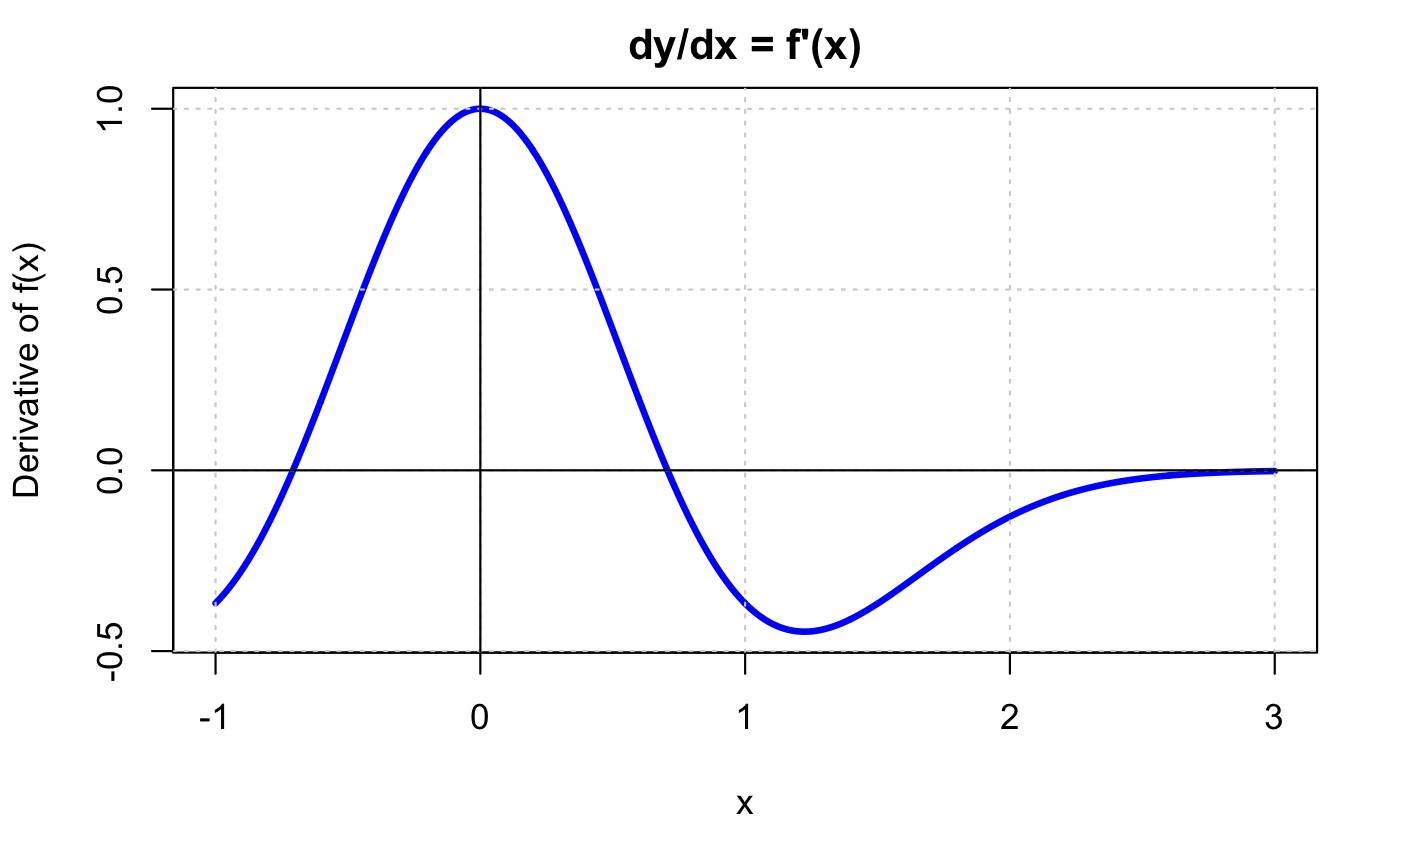
\includegraphics[width=.99\linewidth]{dy_dx.png}
     \caption{$f^{\prime}(x)$ computed by our function D}\label{Fig:Data2}
   \end{minipage}
\end{figure}


\section{Newton's Method}

\subsection{Overview}

The Derivative function can be applied to Newton's method, which utilizes the derivative of a function to compute its root. Newton's method starts with an initial guess, finds the tangent line to the function at that point and then computes the root of that line. It uses this root as the next guess and repeats this process until a maximum number of iterations is reached or the change between iterations is less than the tolerance.

\subsection{Implementation}

\begin{lstlisting}
Newton <- function(f, x_0, num.its = 40,tol=0.5*10^-10) {
  history = rep(NA, num.its + 1)
  history[1] = x_0
  i = 0
  fprime = D(f)
  while (i < num.its ) {
    i = i + 1
    x_0 = x_0 - f(x_0)/fprime(x_0)
    history[i+1] = x_0
    if (abs(history[i + 1] - abs(history[i])) < tol)
      break
  }
  return(list(root=x_0,history=history[!is.na(history)]))
 }
\end{lstlisting}

\subsection{Testing}
We test the improved Newton's method code on the function $f(x) = \cos(x)^2 + \sin(x) - 1$ with the root at $ x = \pi$. With an initial guess of 4, our newton's method converges super-linearly to the root $\pi$ in 7 iterations. This root has an error of $7.1 \times 10^{-15}$, which is on the order of machine epsilon. \\

\noindent For some functions, however, Newton's method does not converge. An example of this is the cycling example $f(x) = 4x^4 - 6x^2 - 11/4$, whose graph is shown below in Figure 3. With an initial guess of $\frac{1}{2}$, Newton's method will bounce between $\frac{1}{2}$ and $-\frac{1}{2}$, and will never converge to a root.

\begin{figure}[H]
$$
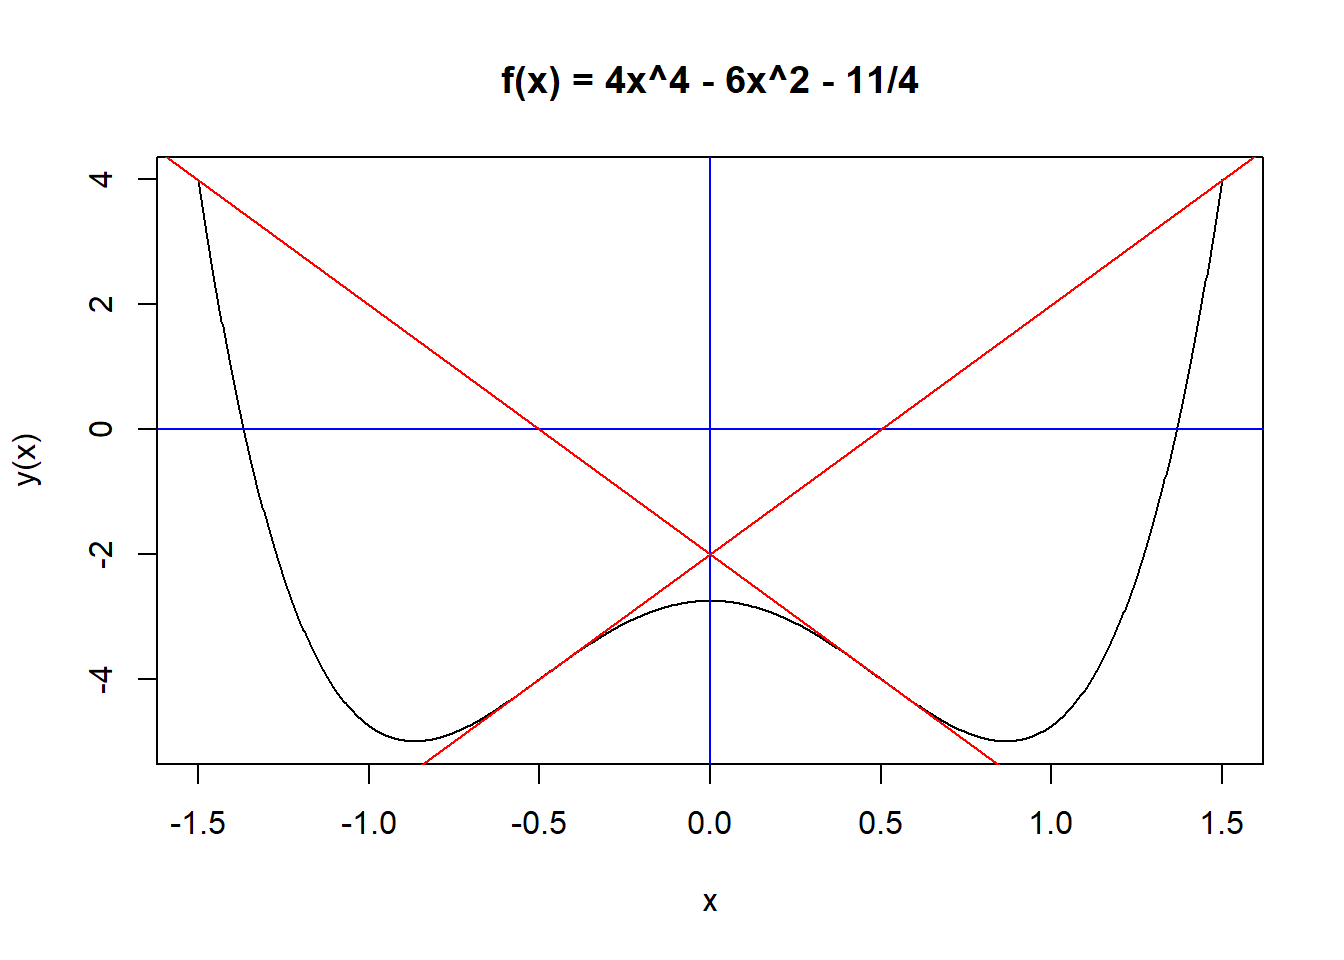
\includegraphics[width=3in]{Q2_2.png} 
$$
\caption{Newton Method Test with $f(x) = 4x^4 - 6x^2 - 11/4$.}
\end{figure}


\section{Optimizing $\delta$ Value}

\subsection{Overview}

Theoretically, the finite difference equation is most accurate when $\delta$ approaches zero. However, this proves to be computationally infeasible because we cannot divide by zero. For this reason, it must be asked: which value of $\delta$ corresponds to the most accurate derivative? 

\subsection{Implementation}

The procedure we take to examine which $\delta$ is the most appropriate consists of: 1. picking a function 2. applying our derivative method to this function with varying $\delta$ values. We then computed the error of each $\delta$ and find out which one yields the least error. We perform this procedure on three functions: $f(x) = e^x$, $g(x) = x^3 + 2x$ and $h(x) = x^8 + 2x - 1$. Our results can be seen in figure 4.

\vspace{1mm}

\begin{lstlisting}
f <- function(x) {exp(x)}
slopes=function(f,x){
  df <- D(f,delta = 10^(-1:-20))
  return(df(x))
}
slopes <- slopes(f,0)  # slope should be 1
error <- abs(slopes - 1)
\end{lstlisting}

\noindent In figure 4a, the log of the error starts to decrease for the three functions as the power of $\delta$ decreases from $-1$ before it reaches $ \approx -8$ (indicating $\delta = 10^{-8}$). Then the error starts to increase again. We zoomed in on the behavior of $\delta$ near $10^{-8}$(shown in figure 4b). From this we concur that the optimal $\delta$ is dependent on the function, but is around $\delta = 10^{-8}$.

\begin{figure}[H]
$$
\begin{minipage}{3in}
\begin{center}
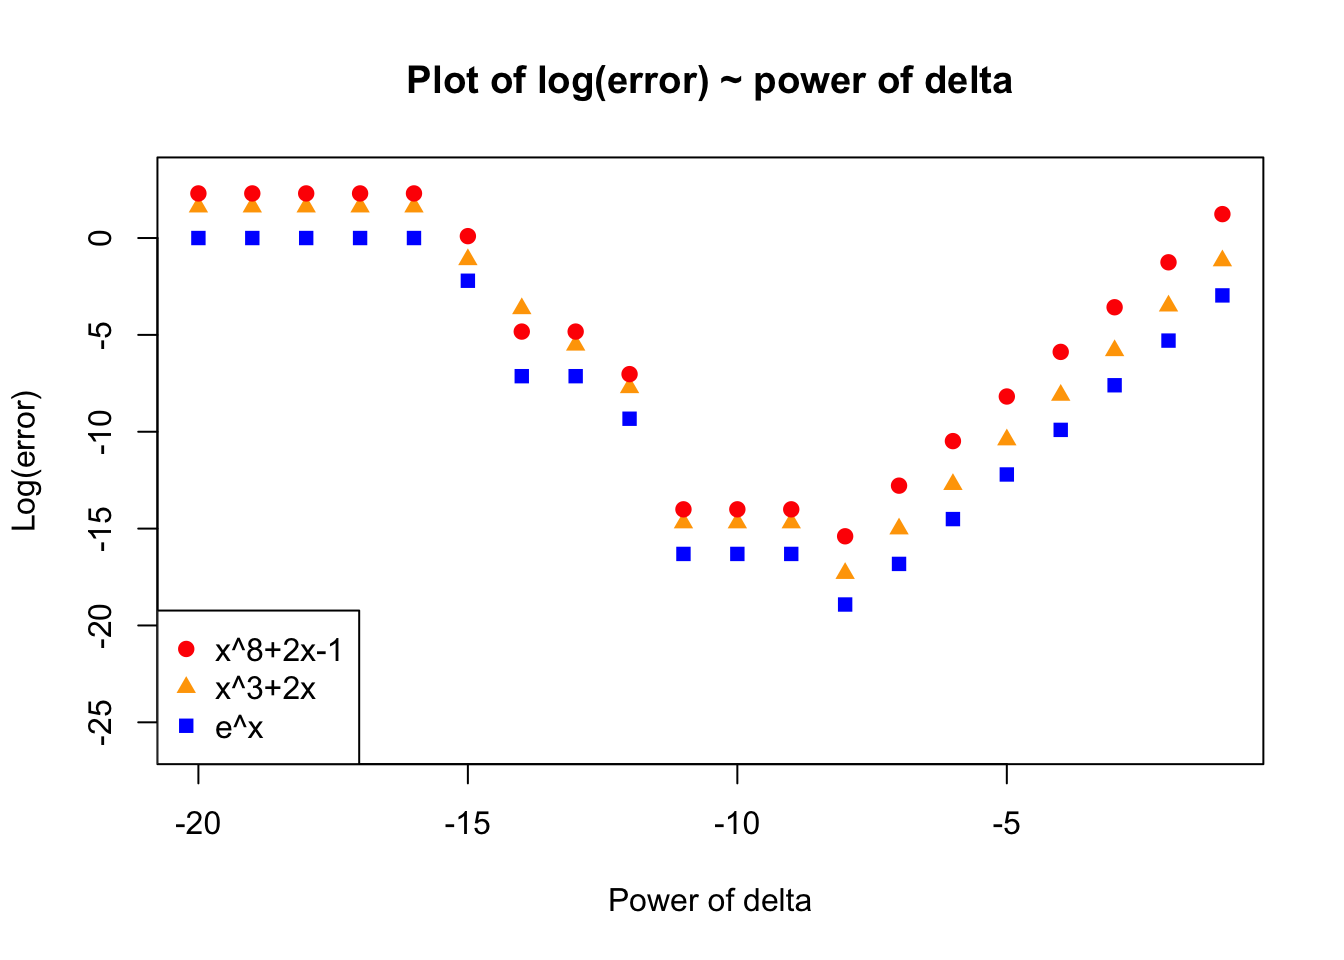
\includegraphics[width=\textwidth]{Q3.1.png} \\
~~~~~(a)
\end{center}
\end{minipage}
\begin{minipage}{3in}
\begin{center}
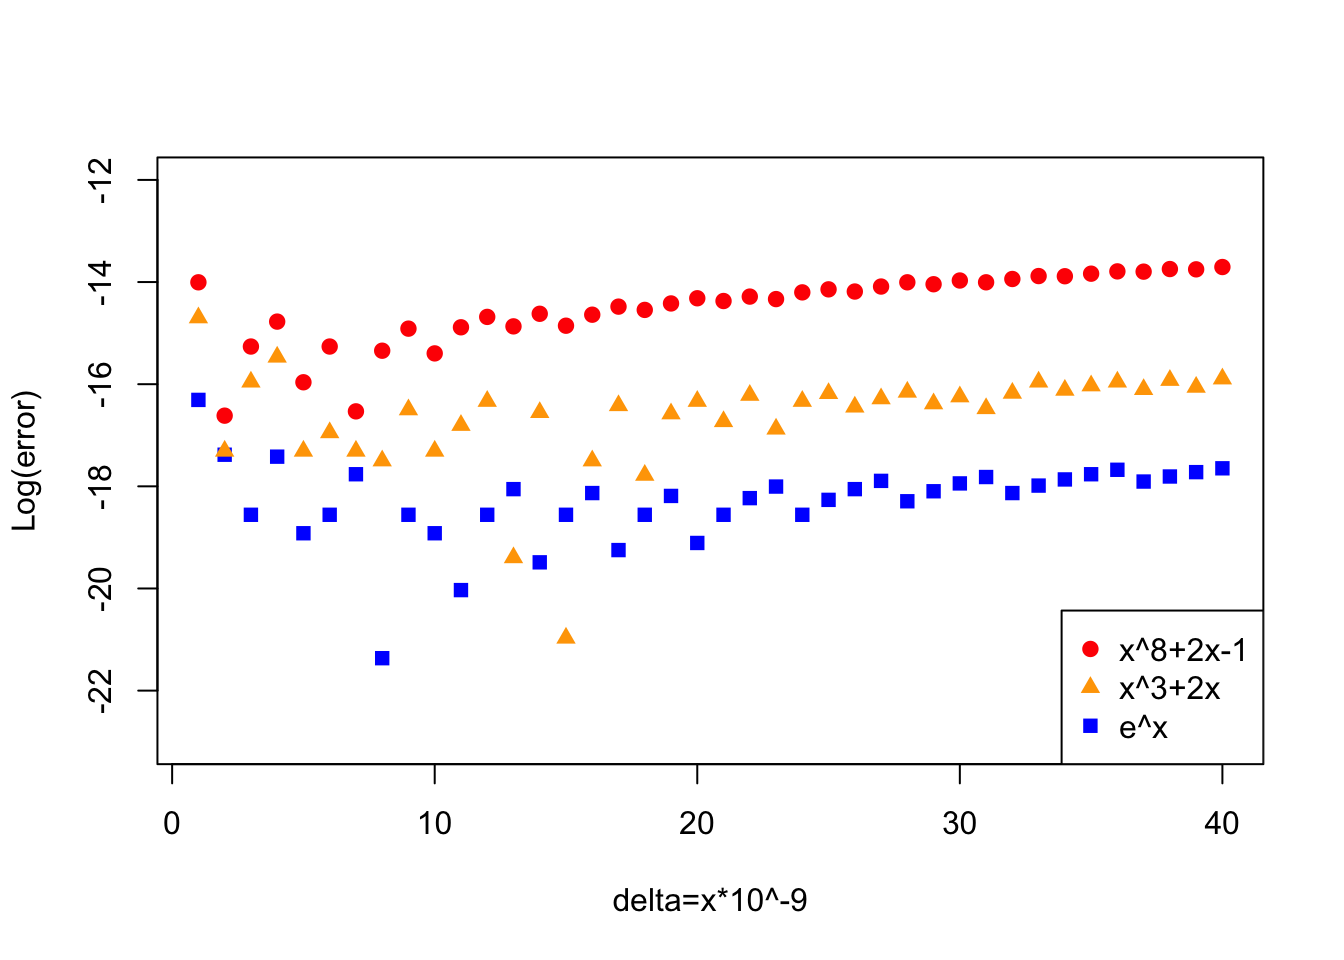
\includegraphics[width=\textwidth]{Q3.2.png} \\
~~~~~(b)
\end{center}
\end{minipage}
$$
\vspace{1mm}
\caption{log error of $\delta$ values for three functions. (a) Behavior of error as the power of $\delta$ decreases. (b) Zoomed-in plot of (a) }
\end{figure} \label{Fig:failure1}

\vspace{3mm}
    
\noindent Interesting to notice, $\delta$ is in the neighborhood of $10^{-8}$ for all 12 polynomial functions we tried. However, $\delta$ behaves differently for trigonometric functions such as $\sin(x)$. See Figure 5.

\begin{figure}[H]
$$
\begin{minipage}{2.85in}
\begin{center}
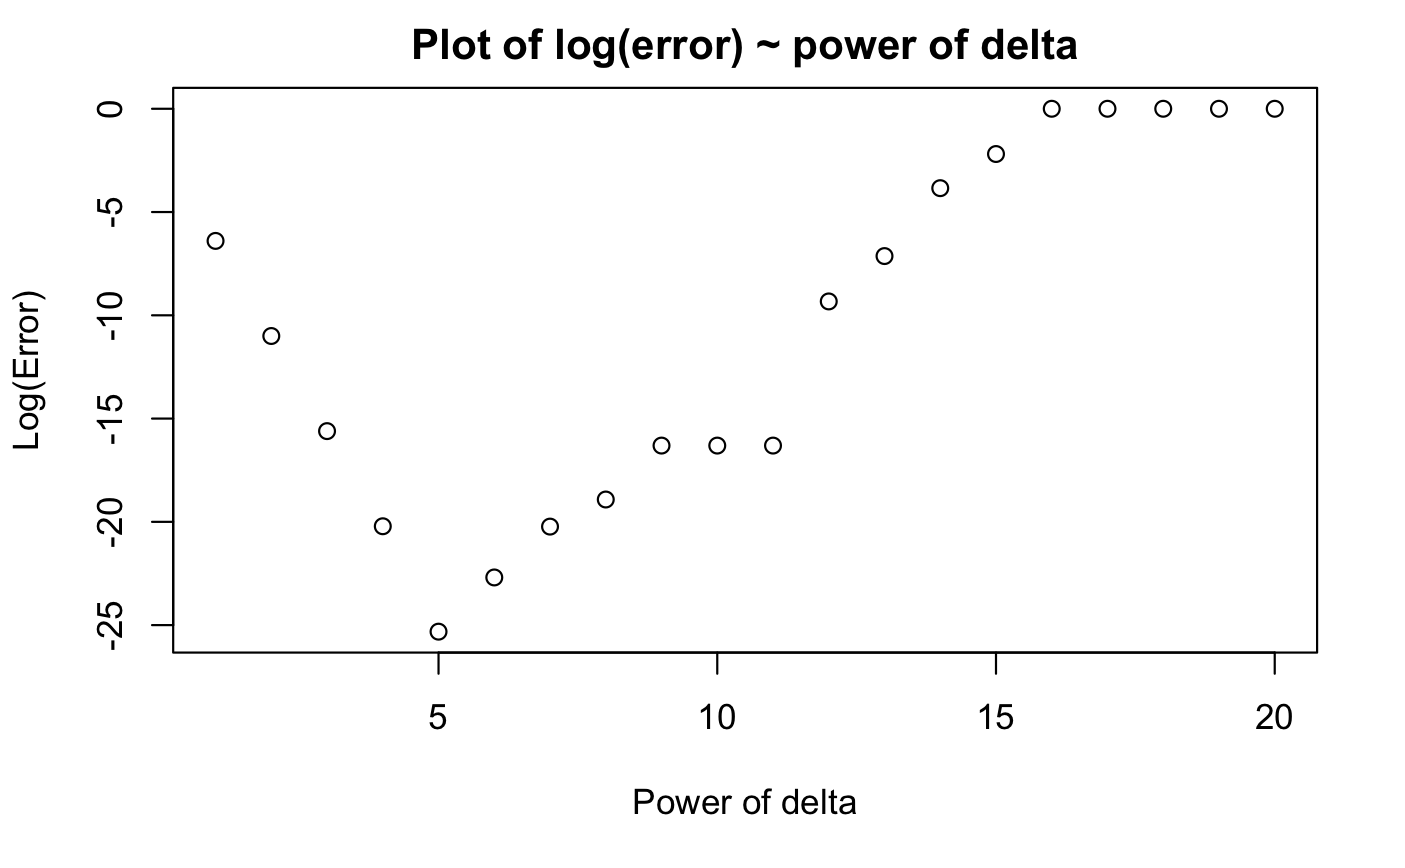
\includegraphics[width=\textwidth]{Q3_5.png} \\
~~~~~(a)
\end{center}
\end{minipage}
\begin{minipage}{2.85in}
\begin{center}
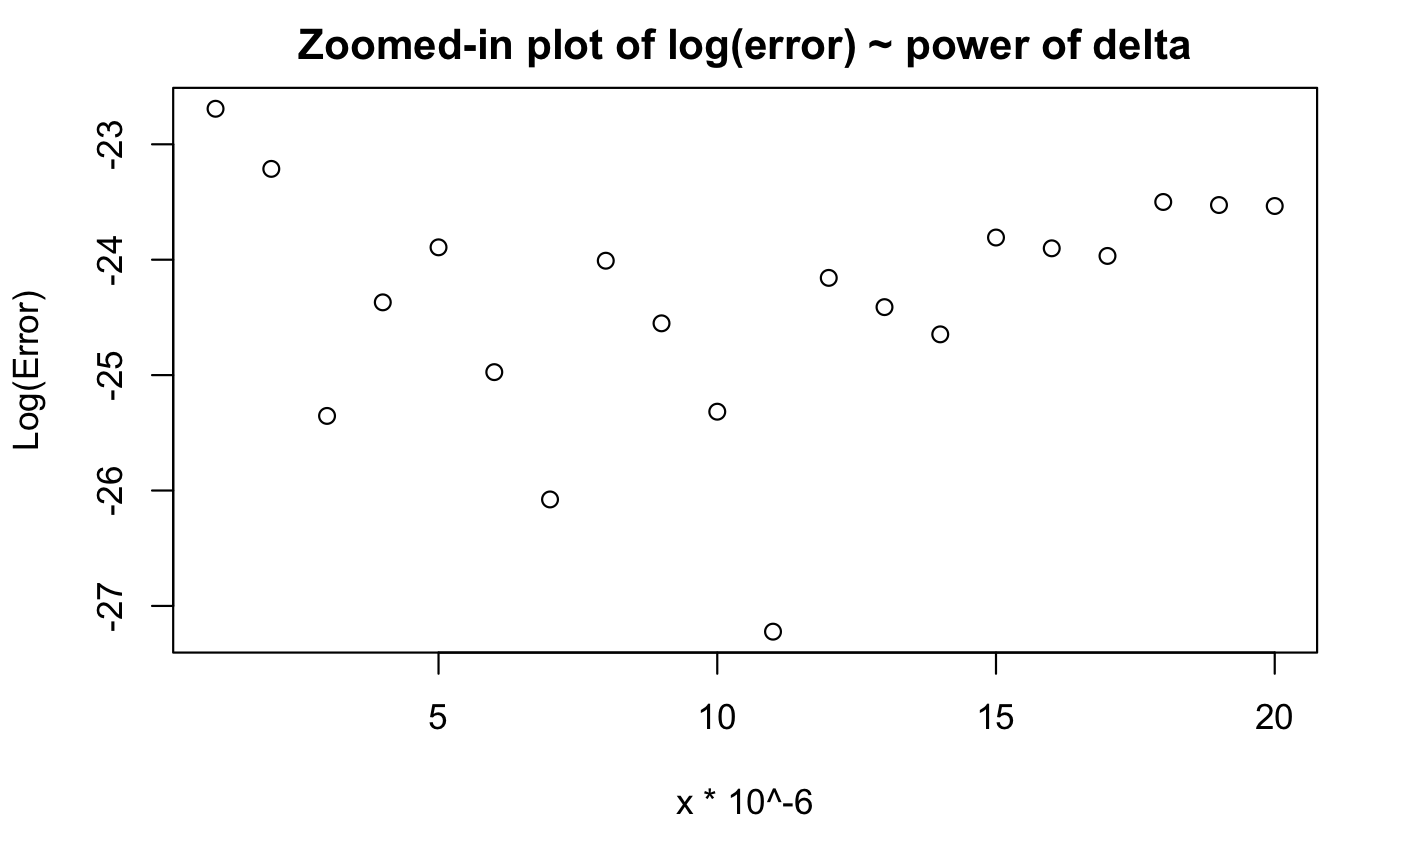
\includegraphics[width=\textwidth]{Q3_6.png} \\
~~~~~(b)
\end{center}
\end{minipage}
$$
\vspace{1mm}
\caption{log error of $\delta$ values for $\sin(x)$. (a) Behavior of error as the power of $\delta$ decreases. (b) Zoomed-in plot of (a) yields $1.1 \times 10^{-5}$.}
\end{figure} \label{Fig:failure1}

\noindent The code below shows how the error for $e^x$ with regards to different values of \(\delta\) is generated. The process for three functions is analogous. See Table 1: delta and error values where the error is minimized.

\begin{lstlisting}
df <- D(f,delta = ((.5+(1:100000)/100000))*10^-8)
error <- abs(df(0)-1)
data.frame("delta"=c(((.5+(1:100000)/100000))*10^-8), "error"=e) %>% 
  arrange(e) %>% 
  head()
\end{lstlisting}

\begin{figure}[H]
$$
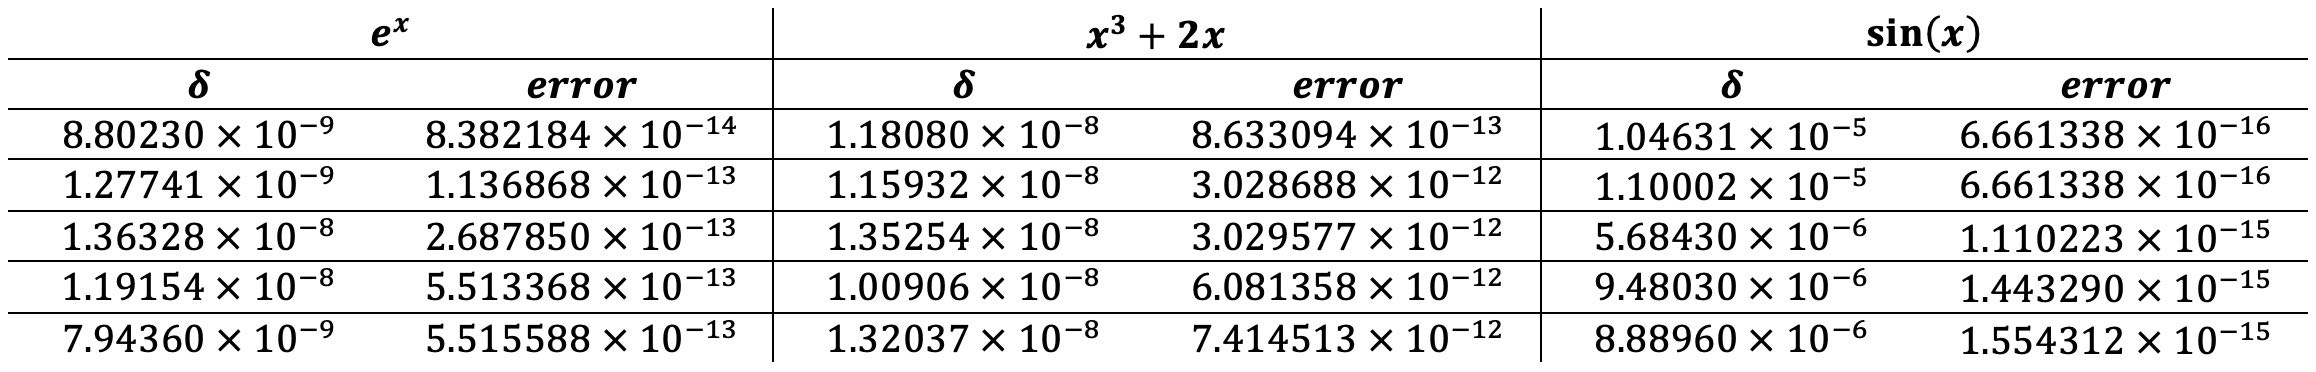
\includegraphics[width=6in]{table.png} 
$$
\centering{Table 1: }{Optimized $\delta$ for three functions correct to 5 decimal places. Left to right: $e^x$, $x^3 + 2x$, $\sin(x)$.}
\end{figure}

\subsection{Result}

Our primary conclusion is that $\delta \approx 10^{-8}$ for polynomial functions, but $\delta$ fluctuates depending on the function it is used on. More specifically, $\delta$ increases to approximately $10^{-5}$ for trigonometric functions such as $\sin(x)$. Although theoretically $E({f'(x + \delta)} - f'(x)) \rightarrow 0$ as $\delta \rightarrow 0$, such behavior of $\delta$ can be considered as a drawback of numerical analysis.


\section{Differences between finite difference methods}
\subsection{Overview}
The finite difference method comes in multiple forms, the forward equation which is featured in section 1 (1.1), the three-point centered difference (4.1), and the backward difference method (4.2).

\begin{center}
$f^{\prime}(x)=\lim \limits_{\delta\rightarrow0}\frac{f(x-\delta)-f(x+\delta)}{2\delta}$ \; \; \; (4.1) \; \; \; \; \; \; \; \; \; \; \; \; \;$f^{\prime}(x)=\lim \limits_{\delta\rightarrow0}\frac{f(x)-f(x-\delta)}{\delta}$ \; \; \; (4.2)
\end{center}

\noindent A visual representation of these equations on an arbitrary function can be found in Figure 6d on the next page. The three methods differ on which points they compute the slope between. The forward difference method uses points x and x + $\delta$, the centered method uses x - $\delta$ and x + $\delta$ and the backwards method uses x - $\delta$ and x.

\subsection{Testing}

In order to test which method produces the least error, we choose two functions, $e^{x}$ and $x^3 + 2x$. We apply each method with different $\delta$ values and subtract the pairwise error. A positive difference leads to a worse performance. Therefore, we can conclude that the forward method has the worst performance. See Figure 6. \\

\noindent It is worth noting that while centered difference method performs better as $\delta \rightarrow 10^{-8}$, it performs worse as the power decreases from $10^{-8}$.

\begin{figure}[H]
$$
\begin{minipage}{2.75in}
\begin{center}
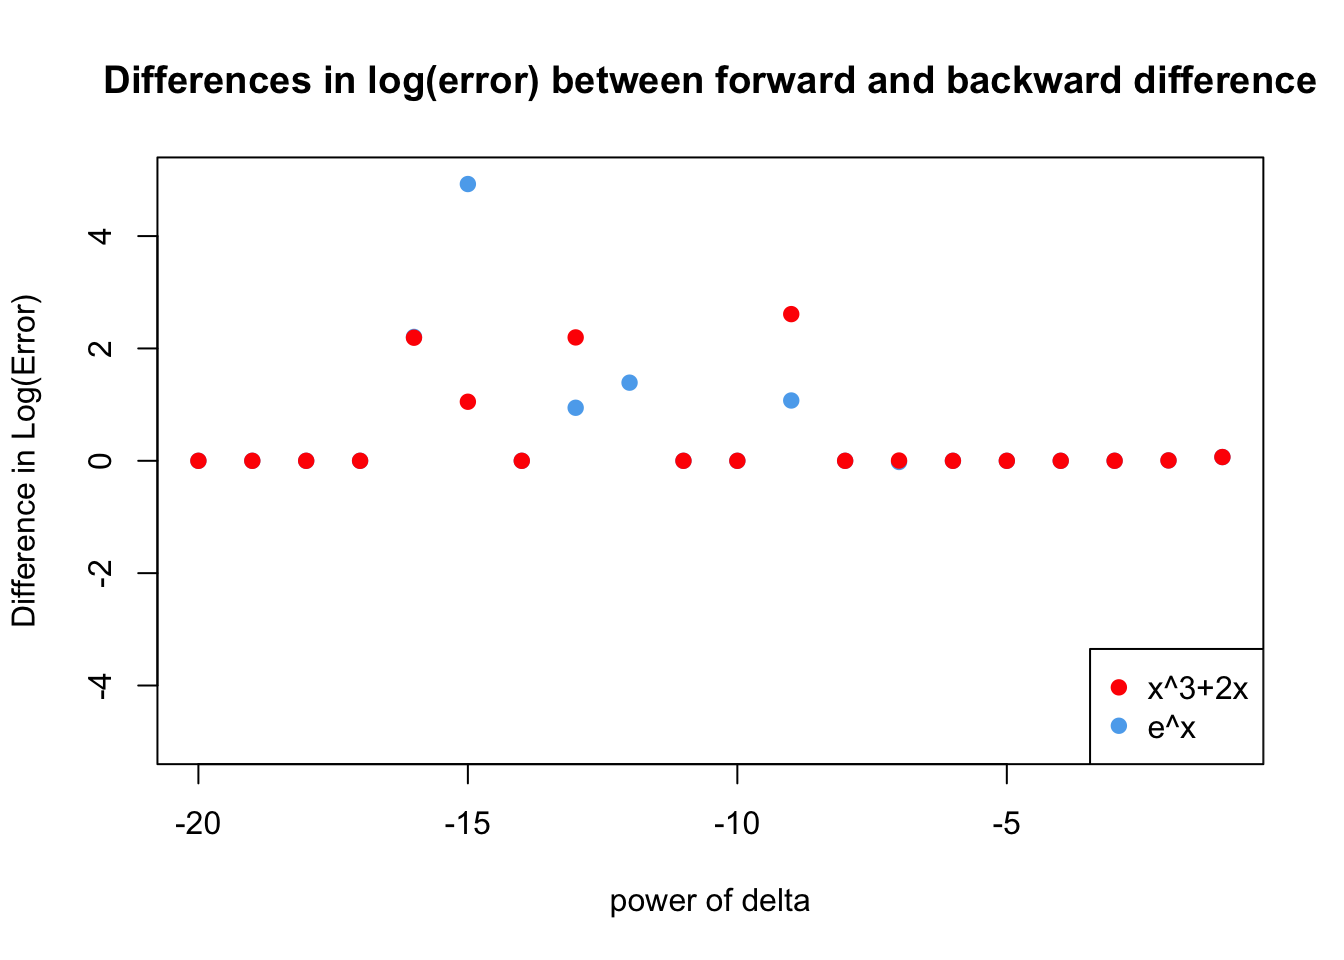
\includegraphics[width=\textwidth]{Q4.1.png} \\
~~~~~(a)
\end{center}
\end{minipage}
\begin{minipage}{2.75in}
\begin{center}
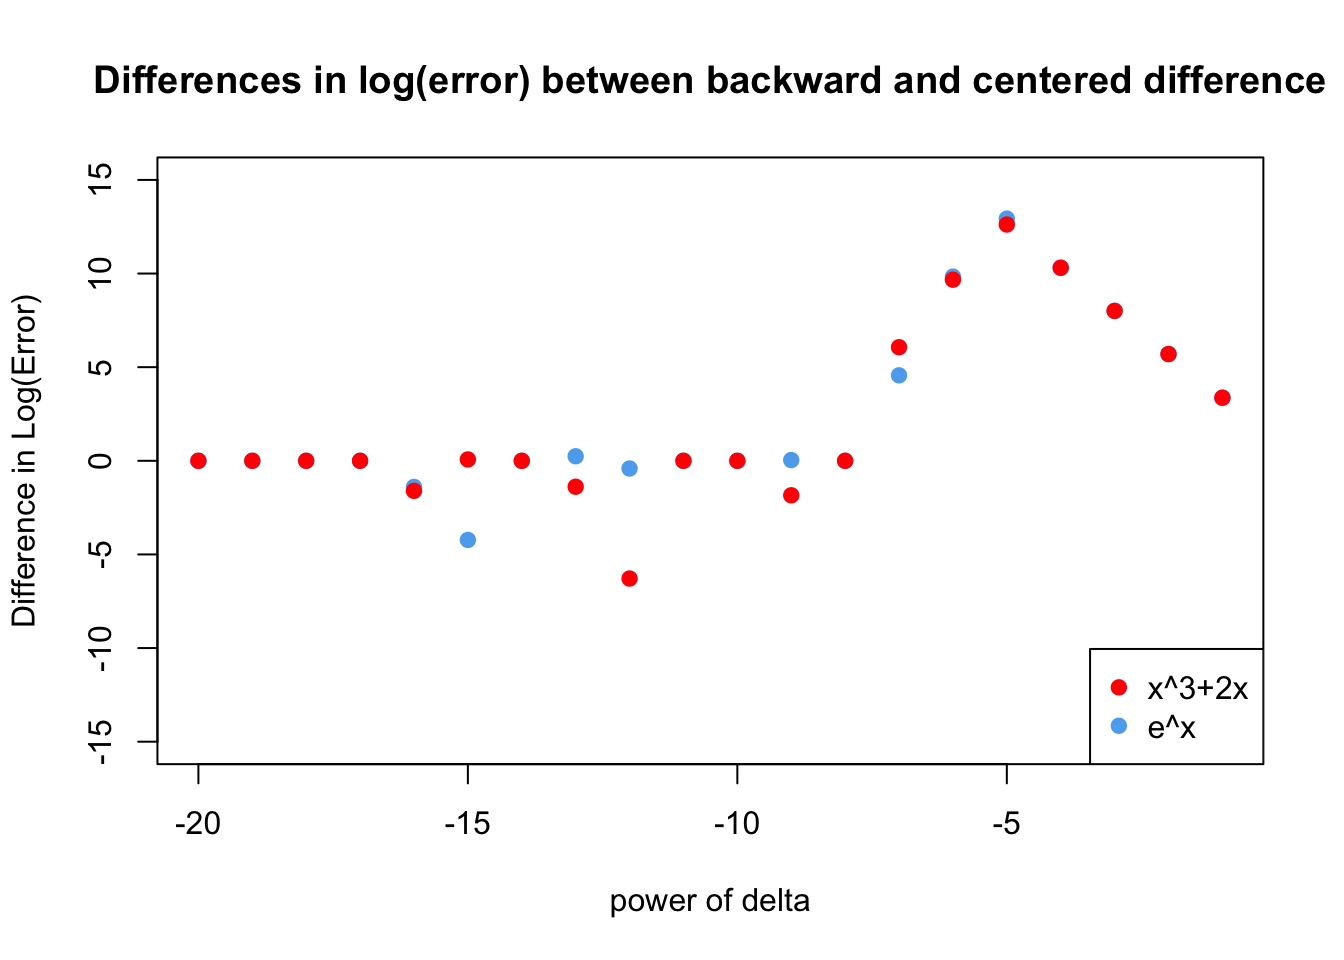
\includegraphics[width=\textwidth]{Q4.2.png} \\
~~~~~(b)
\end{center}
\end{minipage}
$$
\end{figure}
\vspace{-10mm}
\begin{figure}[H]
$$
\begin{minipage}{2.75in}
\begin{center}
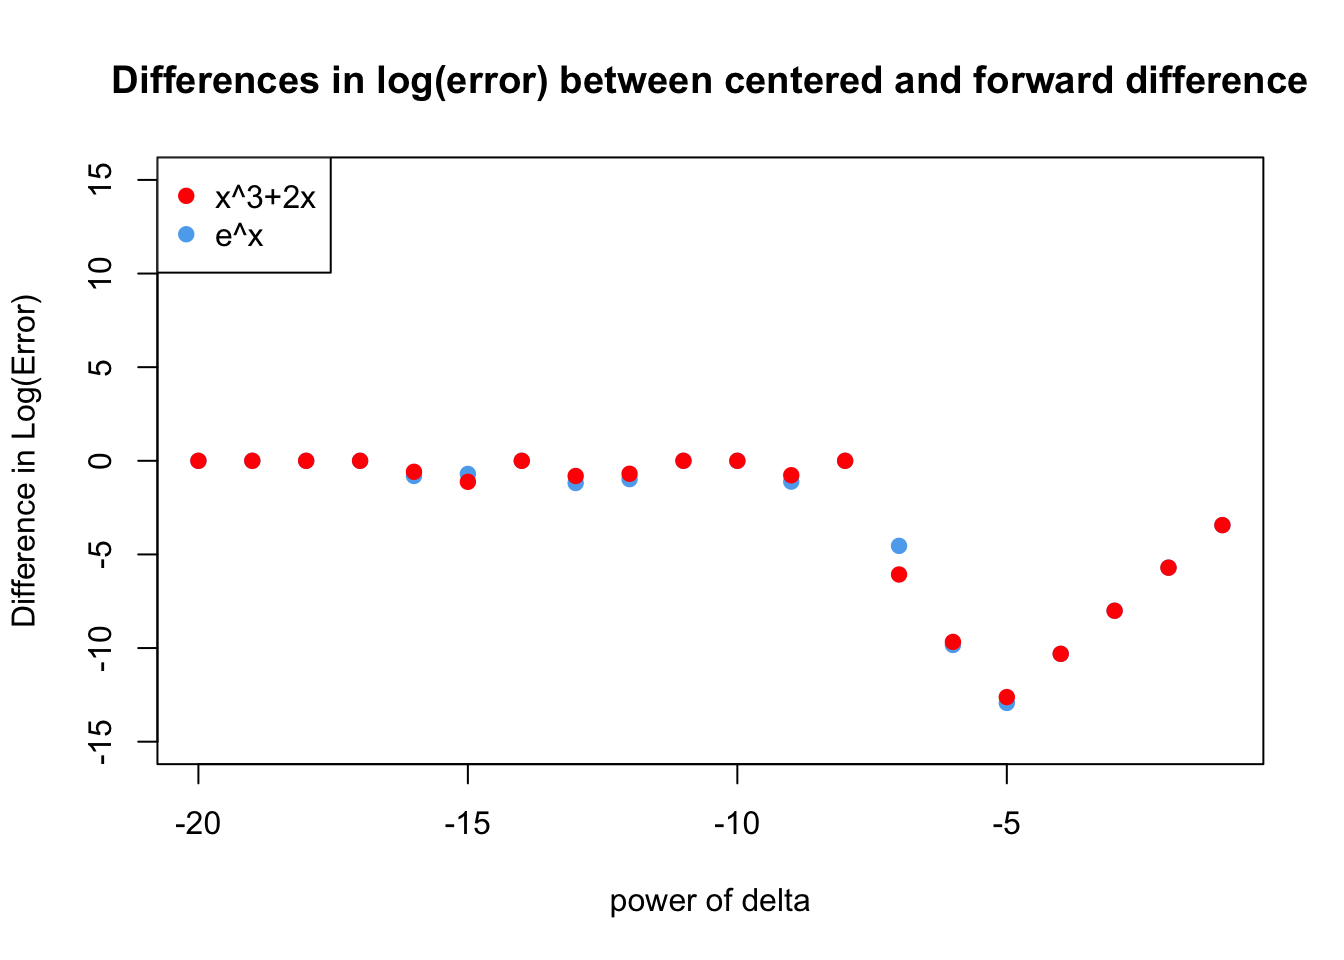
\includegraphics[width=\textwidth]{Q4.3.png} \\
~~~~~(c)
\end{center}
\end{minipage}
\begin{minipage}{2.75in}
\begin{center}
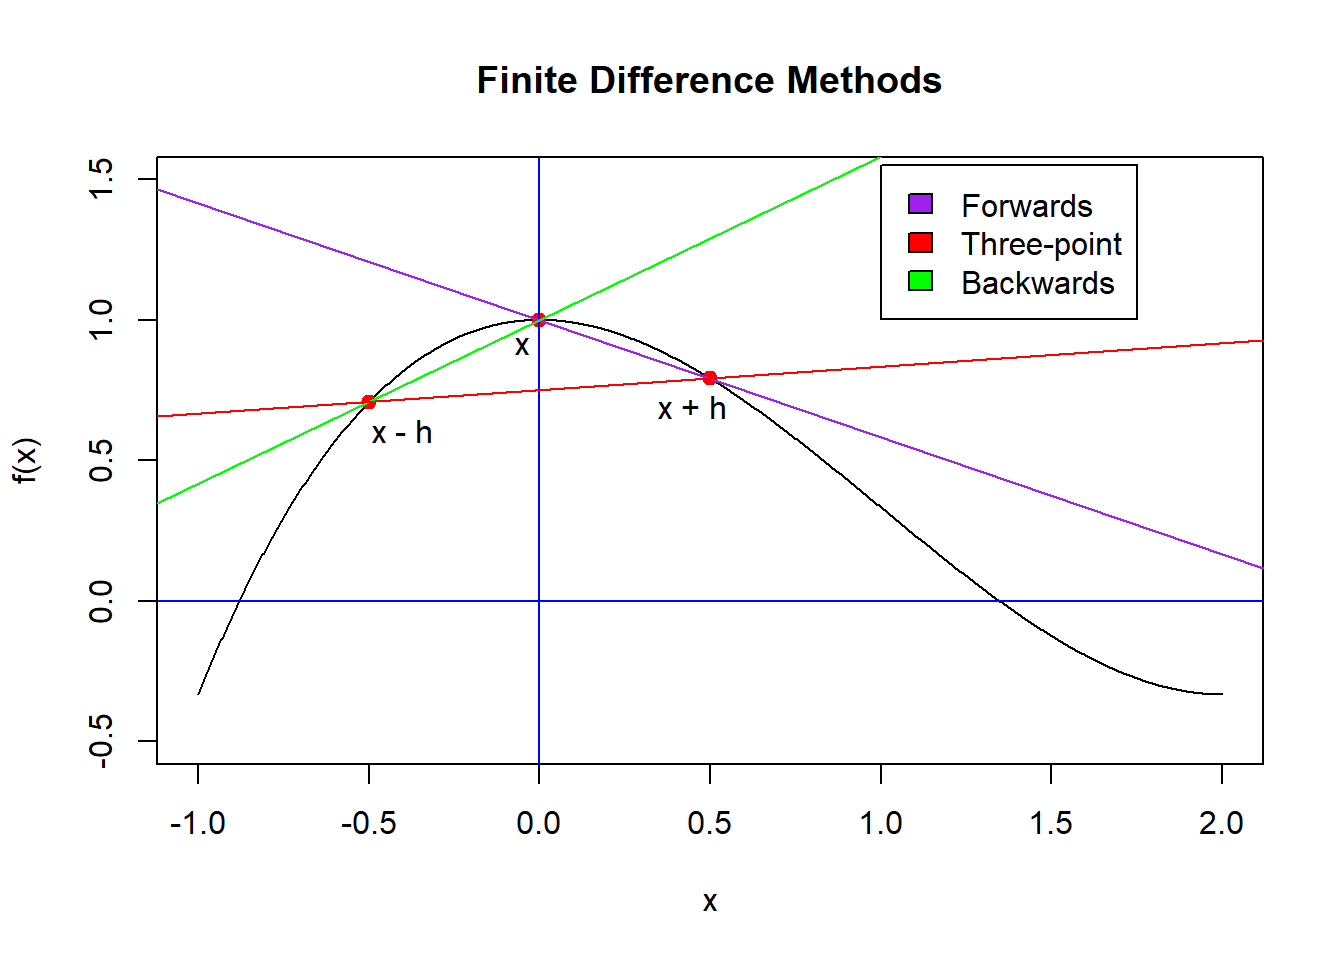
\includegraphics[width=\textwidth]{FiniteDifferenceMethods.png} \\
~~~~~(d) Visualization representation of three finite difference methods
\end{center}
\end{minipage}
\vspace{3mm}
\caption{Pairwise difference in log(error)} 
$$
\end{figure} \label{Fig:failure1}

\vspace{-10mm}

\section*{Conclusion}
Theoretically, we should have more precise results from the different methods of differentiation by decreasing $\delta$. However, the opposite is true due to rounding errors. As rounding errors are inevitable in numerical differentiation, there is a threshold for how small $\delta$ can get depending on the input functions we choose. In this report, we have shown that the smallest $\delta$ value for the least errors for $e^x$, $x^3 + 2x$ and sin(x) are, respectively, $8.80230 \times 10^{-8}$, $1.18080 \times 10^{-8}$ and $1.04631 \times 10^{-5}$.  \\

\noindent Furthermore, the graphs of log(errors) for these 3 functions affirm our prediction that as $\delta$ exceeds the threshold respectively, error starts to increase. By plotting the difference errors resulted from these two methods to $\delta$ value, we also found that the three-point centered-difference method provides more precise result compared with the two-point forward-difference method. This can be explained by that $\delta$ can be approximately as small as the cubic root of $\epsilon_{\text{machine}}$ for the first method, while it can only be as small as the square root for $\epsilon_{\text{machine}}$ for the latter. Due to this reason, for future work we can explore how threshold for $\delta$ of three-point centered-difference method to find the characteristics of a function that determine its optimal $\delta$ value.

\end{document}